%\RequirePackage[l2tabu, orthodox]{nag}
\RequirePackage{currfile}
\documentclass[12pt]{beamer}
\graphicspath{{Imagenes/}{../Imagenes/}}
\usepackage[utf8]{inputenc}
\usepackage[spanish]{babel}
\usepackage{standalone}
\usepackage{color}
\usepackage[binary-units=true]{siunitx}
\usepackage{hyperref}
\hypersetup{
  colorlinks=true,
  linkcolor=blue,          % color of internal links (change box color with linkbordercolor)
  citecolor=green,        % color of links to bibliography
  filecolor=magenta,      % color of file links
  urlcolor=cyan,           % color of external links
  linkbordercolor={0 0 1}
}
\usepackage{xcolor, soul}
\usepackage{etoolbox}
\usepackage{amsmath}
\usepackage{amsthm}
\usepackage{physics}
\usepackage{multicol}
\usepackage{graphicx}
\usepackage{bookmark}
\usepackage{longtable}
\usepackage{graphicx}
\usepackage{tikz}
\usepackage[siunitx, RPvoltages]{circuitikz}
\usetikzlibrary{mindmap}
\usetikzlibrary{arrows, patterns, shapes, decorations.markings, decorations.pathmorphing}
\usetikzlibrary{matrix,positioning}
\tikzstyle{every picture}+=[remember picture,baseline]
\usepackage[autostyle,spanish=mexican]{csquotes}
\usepackage{pifont}
\usepackage[font=footnotesize,textfont=it]{caption}
\usepackage{tabulary}
\usepackage{booktabs}
\usepackage[outdir=./]{epstopdf}
%\usepackage{epstopdf}
\usepackage{media9}
\usepackage{multimedia}
\usepackage{bigints}
%\usepackage{enumitem}
\usepackage[os=win]{menukeys}
\usepackage{pifont}
\usepackage{pbox}
\usepackage{alltt}
\usepackage{verbatim}
\usepackage{colortbl}
\usepackage{tcolorbox}
\usepackage{fancyvrb}
\usepackage[sfdefault]{roboto}  %% Option 'sfdefault' only if the base font of the document is to be sans serif
%\usepackage[T1]{fontenc}
\setcounter{secnumdepth}{3}
\setcounter{tocdepth}{3}
\DeclareGraphicsExtensions{.pdf,.png,.jpg}
\renewcommand {\arraystretch}{1.5}
\definecolor{ao}{rgb}{0.0, 0.5, 0.0}
\definecolor{aquamarine}{rgb}{0.5, 1.0, 0.83}
\definecolor{kellygreen}{rgb}{0.3, 0.73, 0.09}
\definecolor{bisque}{rgb}{1.0, 0.89, 0.77}
\definecolor{amber}{rgb}{1.0, 0.75, 0.0}
\definecolor{armygreen}{rgb}{0.29, 0.33, 0.13}
\definecolor{alizarin}{rgb}{0.82, 0.1, 0.26}
\definecolor{cadetblue}{rgb}{0.37, 0.62, 0.63}
\newcommand*{\TitleParbox}[1]{\parbox[c]{6cm}{\raggedright #1}}%
\newcommand{\python}{\texttt{python}}
\newcommand{\textoazul}[1]{\textcolor{blue}{#1}}
\newcommand{\azulfuerte}[1]{\textcolor{blue}{\textbf{#1}}}
\newcommand{\funcionazul}[1]{\textcolor{blue}{\textbf{\texttt{#1}}}}
%\normalfont
\usepackage{ccfonts}% http://ctan.org/pkg/{ccfonts}
\usepackage[T1]{fontenc}% http://ctan.or/pkg/fontenc
\renewcommand{\rmdefault}{cmr}% cmr = Computer Modern Roman
\usefonttheme[onlymath]{serif}
\linespread{1.3}
\newcounter{saveenumi}
\newcommand{\seti}{\setcounter{saveenumi}{\value{enumi}}}
\newcommand{\conti}{\setcounter{enumi}{\value{saveenumi}}}
\newcommand{\tikzmark}[1]{\tikz[remember picture] \node[coordinate] (#1) {#1};}

\usepackage{scalerel}[2016-12-29]
\def\stretchint#1{\vcenter{\hbox{\stretchto[440]{\displaystyle\int}{#1}}}}
\def\scaleint#1{\vcenter{\hbox{\scaleto[3ex]{\displaystyle\int}{#1}}}}
\def\bs{\mkern-12mu}

\newtheorem{teo}{}[section]
\usepackage{blkarray}

%reduce el tamaño de letra de la etiqueta equations
\makeatletter
\def\maketag@@@#1{\hbox{\m@th\normalfont\small#1}}
\makeatother

%se usa para la x en itemize
\newcommand{\xmark}{\text{\ding{55}}}

%\AtBeginDocument{\setlength{\tymin}{1em}}


\definecolor{myblue}{rgb}{.8, .8, 1}

\usepackage{empheq}

\newlength\mytemplen
\newsavebox\mytempbox

\makeatletter
\newcommand\mybluebox{%
    \@ifnextchar[%]
       {\@mybluebox}%
       {\@mybluebox[0pt]}}

\def\@mybluebox[#1]{%
    \@ifnextchar[%]
       {\@@mybluebox[#1]}%
       {\@@mybluebox[#1][0pt]}}

\def\@@mybluebox[#1][#2]#3{
    \sbox\mytempbox{#3}%
    \mytemplen\ht\mytempbox
    \advance\mytemplen #1\relax
    \ht\mytempbox\mytemplen
    \mytemplen\dp\mytempbox
    \advance\mytemplen #2\relax
    \dp\mytempbox\mytemplen
    \colorbox{myblue}{\hspace{1em}\usebox{\mytempbox}\hspace{1em}}}

\makeatother



%Se usa la plantilla Warsaw modificada con whale
\mode<presentation>
{
  \usetheme{Warsaw}
  \setbeamertemplate{headline}{}
  %\useoutertheme{infolines}
  \usecolortheme{whale}
  \setbeamercovered{invisible}
  

 \setbeamertemplate{section in toc}[sections numbered]
 \setbeamertemplate{subsection in toc}[subsections numbered]
 \setbeamertemplate{subsection in toc}{\leavevmode\leftskip=3.2em\rlap{\hskip-2em\inserttocsectionnumber.\inserttocsubsectionnumber}\inserttocsubsection\par}
% \setbeamercolor{section in toc}{fg=blue}
 \setbeamercolor{subsection in toc}{fg=blue}
 \setbeamerfont{subsection in toc}{size=\small}


\setbeamertemplate{navigation symbols}{}
\setbeamertemplate{caption}[numbered]
% \setbeamercolor{frametitle}{fg=yellow,bg=blue!70!white}
\setbeamercolor{section in head/foot}{bg=black, fg=white}
%\setbeamercolor{subsection in head/foot}{bg=gray!30,fg=black}
%\setbeamercolor{author in head/foot}{fg=yellow}
%\setbeamercolor{date in head/foot}{fg=blue}

%\mode<presentation>
%{
%  \usetheme{Warsaw}
%  \setbeamertemplate{headline}{}
%  %\useoutertheme{infolines}
%  \useoutertheme{default}
%  \setbeamercovered{invisible}
%  % or whatever (possibly just delete it)
%}
}


\usepackage{courier}
\usepackage{listingsutf8}
\usepackage{listings}
\usepackage{xcolor}
\usepackage{textcomp}
\usepackage{color}
\definecolor{deepblue}{rgb}{0,0,0.5}
\definecolor{brown}{rgb}{0.59, 0.29, 0.0}
\definecolor{OliveGreen}{rgb}{0,0.25,0}
% \usepackage{minted}

\DeclareCaptionFont{white}{\color{white}}
\DeclareCaptionFormat{listing}{\colorbox{gray}{\parbox{0.98\textwidth}{#1#2#3}}}
\captionsetup[lstlisting]{format=listing,labelfont=white,textfont=white}
\renewcommand{\lstlistingname}{Código}


\definecolor{Code}{rgb}{0,0,0}
\definecolor{Keywords}{rgb}{255,0,0}
\definecolor{Strings}{rgb}{255,0,255}
\definecolor{Comments}{rgb}{0,0,255}
\definecolor{Numbers}{rgb}{255,128,0}

\makeatletter

\newif\iffirstchar\firstchartrue
\newif\ifstartedbyadigit
\newif\ifprecededbyequalsign

\newcommand\processletter
{%
  \ifnum\lst@mode=\lst@Pmode%
    \iffirstchar%
        \global\startedbyadigitfalse%
      \fi
      \global\firstcharfalse%
    \fi
}

\newcommand\processdigit
{%
  \ifnum\lst@mode=\lst@Pmode%
      \iffirstchar%
        \global\startedbyadigittrue%
      \fi
      \global\firstcharfalse%
  \fi
}

\lst@AddToHook{OutputOther}%
{%
  \lst@IfLastOtherOneOf{=}
    {\global\precededbyequalsigntrue}
    {}%
}

\lst@AddToHook{Output}%
{%
  \ifprecededbyequalsign%
      \ifstartedbyadigit%
        \def\lst@thestyle{\color{orange}}%
      \fi
    \fi
  \global\firstchartrue%
  \global\startedbyadigitfalse%
  \global\precededbyequalsignfalse%
}

\lstset{ 
language=Python,                % choose the language of the code
basicstyle=\footnotesize\ttfamily,       % the size of the fonts that are used for the code
numbers=left,                   % where to put the line-numbers
numberstyle=\scriptsize,      % the size of the fonts that are used for the line-numbers
stepnumber=1,                   % the step between two line-numbers. If it is 1 each line will be numbered
numbersep=5pt,                  % how far the line-numbers are from the code
backgroundcolor=\color{white},  % choose the background color. You must add \usepackage{color}
showspaces=false,               % show spaces adding particular underscores
showstringspaces=false,         % underline spaces within strings
showtabs=false,                 % show tabs within strings adding particular underscores
frame=single,   		% adds a frame around the code
tabsize=2,  		% sets default tabsize to 2 spaces
captionpos=t,   		% sets the caption-position to bottom
breaklines=true,    	% sets automatic line breaking
breakatwhitespace=false,    % sets if automatic breaks should only happen at whitespace
escapeinside={\#},  % if you want to add a comment within your code
stringstyle =\color{OliveGreen},
%otherkeywords={{as}},             % Add keywords here
keywordstyle = \color{blue},
commentstyle = \color{black},
identifierstyle = \color{black},
literate=%
         {á}{{\'a}}1
         {é}{{\'e}}1
         {í}{{\'i}}1
         {ó}{{\'o}}1
         {ú}{{\'u}}1
%
%keywordstyle=\ttb\color{deepblue}
%fancyvrb = true,
}

\lstdefinestyle{FormattedNumber}{%
    literate={0}{{\textcolor{red}{0}}}{1}%
             {1}{{\textcolor{red}{1}}}{1}%
             {2}{{\textcolor{red}{2}}}{1}%
             {3}{{\textcolor{red}{3}}}{1}%
             {4}{{\textcolor{red}{4}}}{1}%
             {5}{{\textcolor{red}{5}}}{1}%
             {6}{{\textcolor{red}{6}}}{1}%
             {7}{{\textcolor{red}{7}}}{1}%
             {8}{{\textcolor{red}{8}}}{1}%
             {9}{{\textcolor{red}{9}}}{1}%
             {.0}{{\textcolor{red}{.0}}}{2}% Following is to ensure that only periods
             {.1}{{\textcolor{red}{.1}}}{2}% followed by a digit are changed.
             {.2}{{\textcolor{red}{.2}}}{2}%
             {.3}{{\textcolor{red}{.3}}}{2}%
             {.4}{{\textcolor{red}{.4}}}{2}%
             {.5}{{\textcolor{red}{.5}}}{2}%
             {.6}{{\textcolor{red}{.6}}}{2}%
             {.7}{{\textcolor{red}{.7}}}{2}%
             {.8}{{\textcolor{red}{.8}}}{2}%
             {.9}{{\textcolor{red}{.9}}}{2}%
             {\ }{{ }}{1}% handle the space
         ,%
          %mathescape=true
          escapeinside={__}
          }



\makeatletter

% \setbeamercolor{subsection in foot}{bg=blue!30!yellow, fg=red}
%\setbeamercolor{footlinecolor}{bg=black,fg=white}
\setbeamertemplate{footline}
{
  \leavevmode%
  \hbox{%
  \begin{beamercolorbox}[wd=.333333\paperwidth,ht=2.25ex,dp=1ex,center]{section in footline}%
    \usebeamerfont{section in foot} \insertsection
  \end{beamercolorbox}}%
  \begin{beamercolorbox}[wd=.333333\paperwidth,ht=2.25ex,dp=1ex,center]{subsection in foot}%
    \usebeamerfont{subsection in foot}  \insertsubsection
  \end{beamercolorbox}%
  \begin{beamercolorbox}[wd=.333333\paperwidth,ht=2.25ex,dp=1ex,right]{date in head/foot}%
    \usebeamerfont{date in head/foot} \insertshortdate{} \hspace*{2em}
    \insertframenumber{} / \inserttotalframenumber \hspace*{2ex} 
  \end{beamercolorbox}}%
  \vskip0pt%
\makeatother
\normalfont
\usepackage{ccfonts}% http://ctan.org/pkg/{ccfonts}
\usepackage[T1]{fontenc}% http://ctan.or/pkg/fontenc
\renewcommand{\rmdefault}{cmr}% cmr = Computer Modern Roman
\linespread{1.3}
\title{Ecuaciones diferenciales ordinarias}
\subtitle{Curso de Física Computacional}
\author{M. en C. Gustavo Contreras Mayén}
\date{\today}
\institute{Facultad de Ciencias - UNAM}
\titlegraphic{
\includegraphics[width=1.75cm]{Imagenes/escudo-facultad-ciencias.jpg}\hspace*{4.75cm}~%
   
\includegraphics[width=1.75cm]{Imagenes/escudo-unam.jpg}
}
\begin{document}
\maketitle
\fontsize{14}{14}\selectfont
\spanishdecimal{.}
\section*{Contenido}
\frame{\tableofcontents[currentsection, hideallsubsections]}
\section{Ecuaciones Diferenciales Ordinarias}
\frame{\tableofcontents[currentsection, hideothersubsections]}
\subsection{Método predictor - corrector}
\begin{frame}
\frametitle{Mejora en el método de Euler}
Una forma práctica de superar la baja precisión del método de Euler es elevar el orden de la aproximación aplicando su variante llamada  \textoazul{método predictor - corrector} de Euler, que opera con dos estimaciones de solución en cada paso de propagación.
\end{frame}
\begin{frame}
\frametitle{Método predictor - corrector}
\begin{align}
\overline{y}_{m + 1} &= y_{m} + h \: f(t_{m}, y_{m}), \hspace{0.3cm} m = 1, 2, 3, \ldots \label{eq:ecuacion_12_17} \\
y_{m + 1} &= y_{m} + \dfrac{h}{2} \: [ f(t_{m}, y_{m}) + f(t_{m} + h, \overline{y}_{m + 1})] \label{eq:ecuacion_12_18}
\end{align}
donde
\setbeamercolor{item projected}{bg=purple!80!white,fg=white}
\setbeamertemplate{enumerate items}[circle]
\begin{enumerate}[<+->]
\item $ \overline{y}_{m + 1}$ es el valor predictor.
\item $y_{m + 1}$ es el valor corregido.
\end{enumerate}
\end{frame}
\begin{frame}
\frametitle{Valor predictor}
El valor predictor de la solución $ \overline{y}_{m + 1}$ se obtiene del método de Euler, de la expresión predictora (ec. \ref{eq:ecuacion_12_17}).
\\
\bigskip
Se utiliza para estimar la propagación de la derivada $f(t_{m} + h, \overline{y}_{m + 1})$
\end{frame}
\begin{frame}
\frametitle{Valor corregido}
El valor de la solución corregido $y_{m + 1}$ se obtiene de la fórmula de corrección (ec. \ref{eq:ecuacion_12_18}), que utiliza el promedio de la derivada estimada 
\[\dfrac{[ f(t_{m}, y_{m}) + f(t_{m} + h, \overline{y}_{m + 1})]}{2}
\]
en el intervalo $[x_{m}, x_{m + 1}]$
\end{frame}
\begin{frame}
\frametitle{Casos especiales de Runge-Kutta}
Veremos más adelante que los métodos de Euler básicos y el predictor - corrector son casos particulares de una familia completa de algoritmos, conocidos como \textoazul{métodos de Runge-Kutta}.
\end{frame}
\begin{frame}
\frametitle{Casos especiales de Runge-Kutta}
El método básico de Euler es equivalente al método de primer orden de Runge-Kutta (RK1).
\\
\bigskip
El algoritmo predictor - corrector de Euler es $O(h^2)$, es equivalente al método de Runge-Kutta de segundo orden (RK2). 
\end{frame}
\begin{frame}
\frametitle{Casos especiales de Runge-Kutta}
La precisión superior del algoritmo predictor-corrector Euler obviamente se produce a expensas de un doble número de evaluaciones de las funciones del lado derecho $f(x, y)$ de las EDO.
\end{frame}
\begin{frame}
\frametitle{Estabilidad y precisión de RK1}
Para revisar la precisión y estabilidad de los métodos de Euler, consideremos el siguiente problema
\begin{align}
y^{\prime \prime} + y &= 0 \label{eq:ecuacion_12_19} \\
y(0) &=  y_{0}, \hspace{0.3cm} y^{\prime}(0) = y^{\prime}_{0} \label{ec:ecuacion_12_20}
\end{align}
\end{frame}
\begin{frame}
\frametitle{Consideraciones}
Obtén la solución a la EDO2 en el intervalo $0 \leq t \leq 100$, con un paso $ht=0.05$.
\end{frame}
\begin{frame}
\frametitle{Solución}
La solución general de este problema es
\[ y(t) = A \: \sin t + B \: \cos t \]
donde las constantes dependen de los valores iniciales $y(0)$, $y^{\prime}_{0}$.
\end{frame}
\begin{frame}
\frametitle{Usando la notación}
Usando la notación descrita anteriormente:
\[ y_{1} \equiv y, \hspace{0.3cm} y_{2} \equiv y^{\prime} \]
por lo que entonces el problema se expresa
\begin{align}
F(x, y) = \begin{bmatrix}
y^{\prime}_{1} &=& y_{2} \\
y^{\prime}_{2} &=& - y{1}
\end{bmatrix}
\end{align}
\end{frame}
\begin{frame}
\frametitle{Usando la notación}
Para las condiciones iniciales:
\begin{align}
\begin{bmatrix}
y_{1}(0) &=& y_{0} \\
y_{2}(0) &=& y^{\prime}_{0}
\end{bmatrix}
\end{align}
\end{frame}
\begin{frame}
\frametitle{Solución exacta}
La solución exacta del problema con los valores iniciales dados:
\[ y_{1}(0) = 0 \hspace{0.3cm} y_{2} = 1 \]
es
\[ y_{1}(t) = \sin t, \hspace{0.3cm} y_{2}(t) = \cos t \]
\end{frame}
\begin{frame}
\frametitle{Código a utilizar}
Usaremos el módulo \funcionazul{moduloEuler} que contiene las funciones \funcionazul{Euler} y \funcionazul{EulerPC}.
\\
\bigskip
Vamos a comparar las dos soluciones.
\end{frame}
\begin{frame}[fragile]
\frametitle{Primera solución}
\begin{lstlisting}[caption=Método de Euler, style=FormattedNumber, basicstyle=\linespread{1.1}\ttfamily=\small, columns=fullflexible]

def Euler(t, ht, y, n, Func):
   f = [0] * (n + 1)

   Func(t, y, f)
   
   for i in range(1, n + 1):
       y[i] += ht * f[i]

   return y
\end{lstlisting}
\end{frame}
\begin{frame}[plain, allowframebreaks, fragile]
\frametitle{Código}
\begin{lstlisting}[caption=Código de Euler, style=FormattedNumber, basicstyle=\linespread{1.1}\ttfamily=\small, columns=fullflexible]
from moduloEuler import Euler, EulerPC

def Func(t, y, f):
   f[_1_] =  y[_2_]
   f[_2_] = -y[_1_]

y0 = 0e0; dy0 = 1e0
tmax = 100e0
ht = 0.05e0

n = 2
y = [_0_]*(n + 1) #componentes de la solucion


t = 0e0
y[_1_] = y_0_
y[_2_] = dy_0_


salida_1_ = open("solucioneuler.txt","w")
salida_1_.write("      t         y_1_        y_2_      check\n")

t = 0e0
y[_1_] = y_0_; y[_2_] = dy_0_

salida_1_.write(("{0:10.5f} {1:10.5f} {2:10.5f} {3:10.5f}\n"). \
          format(t, y[_1_], y[_2_], y[_1_] * y[_1_] + y[_2_] * y[_2_]))

while (t + ht <= tmax):
   Euler(t, ht, y, n, Func)
   t += ht

   salida_1_.write(("{0:10.5f}{1:10.5f}{2:10.5f}{3:10.5f}\n"). \
             format(t,y[_1_], y[_2_], y[_1_] * y[_1_] + y[_2_] * y[_2_]))
salida_1_.close()
\end{lstlisting}
\end{frame}
\begin{frame}[allowframebreaks, plain, fragile]
\frametitle{Código para graficar}
Cómo se genera un archivo de datos, tendremos que recuperar los mismos y luego graficar.
\begin{lstlisting}[caption=Código para graficar, style=FormattedNumber, basicstyle=\linespread{1.1}\ttfamily=\small, columns=fullflexible]

import matplotlib.pyplot as plt

with open('solucioneuler.txt') as f:
    next(f)
    lines = f.readlines()
    t = [float(line.split()[_0_]) for line in lines]
    y = [float(line.split()[_1_]) for line in lines]
    y_2_ = [float(line.split()[_2_]) for line in lines]

plt.figure(1)
plt.plot(t, y)
plt.axhline(y=0, lw=0.75, ls='dashed', color='k')
plt.title('Solucion de la EDO con Euler')
plt.xlabel('tiempo')
plt.ylabel('y')
plt.xlim([0,100])
plt.show()
\end{lstlisting}
\end{frame}
\begin{frame}[plain]
\frametitle{Gráfica de la solución}
\begin{figure}
	\centering
	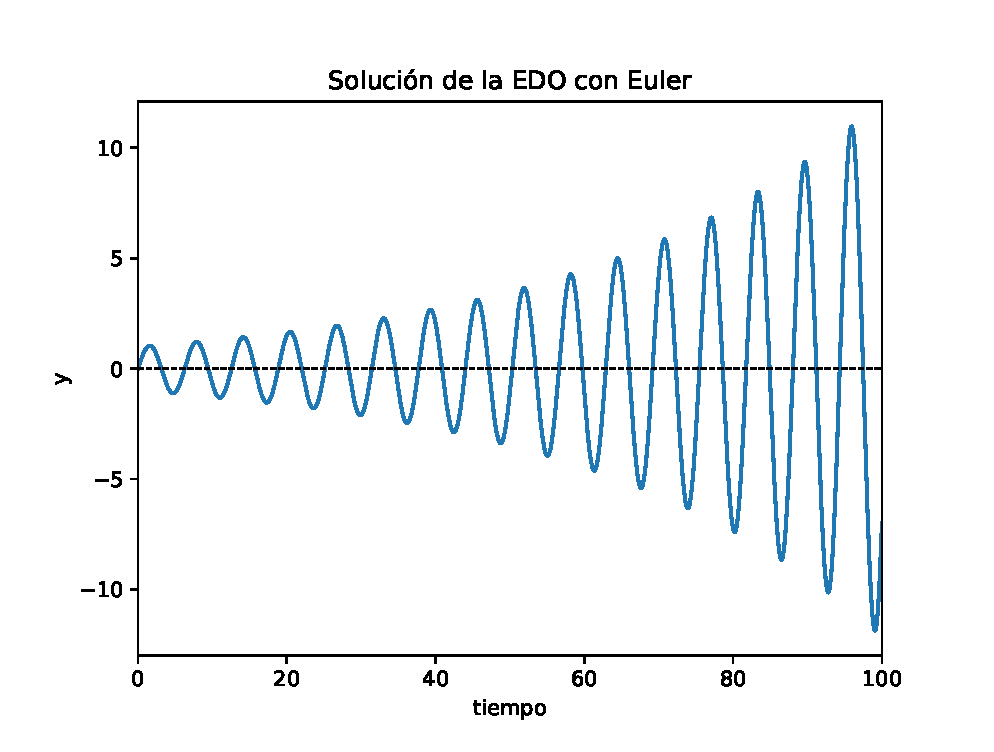
\includegraphics[scale=0.65]{Imagenes/solucion_euler_01.eps}
\end{figure}
\end{frame}
\begin{frame}
\frametitle{¿Qué está ocurriendo?}
Sabemos que la solución de la EDO2 es periódica, no hay factores de amortiguamiento ni otro elemento que modifique la amplitud de la solución.
\\
\bigskip
Pero vemos en la gráfica que aumenta la amplitud conforme transcurre el tiempo.
\end{frame}
\begin{frame}
\frametitle{Diagrama espacio - fase}
Otra manera de revisar si hay una inconsistencia con nuestros resultados, la encontraremos al graficar el estado fase.
\end{frame}
\begin{frame}
\frametitle{Cómo debe de ser}
El estado fase de la EDO2 supone que no hay pérdida de energía, por lo que tendríamos una gráfica cerrada y de trazo uniforme.
\\
\bigskip
Veamos el resultado
\end{frame}
\begin{frame}[allowframebreaks, plain, fragile]
\frametitle{Código para graficar}
Cómo se genera un archivo de datos, tendremos que recuperar los mismos y luego graficar.
\begin{lstlisting}[caption=Código para graficar, style=FormattedNumber, basicstyle=\linespread{1.1}\ttfamily=\small, columns=fullflexible]
plt.figure(_2_)
plt.plot(y, y_2_)
plt.title('Diagrama fase de la EDO')
plt.xlabel('y')
plt.ylabel('$y^{\prime}$')

plt.show()
\end{lstlisting}
\end{frame}
\begin{frame}[plain]
\frametitle{Gráfica del espacio fase}
\begin{figure}
	\centering
	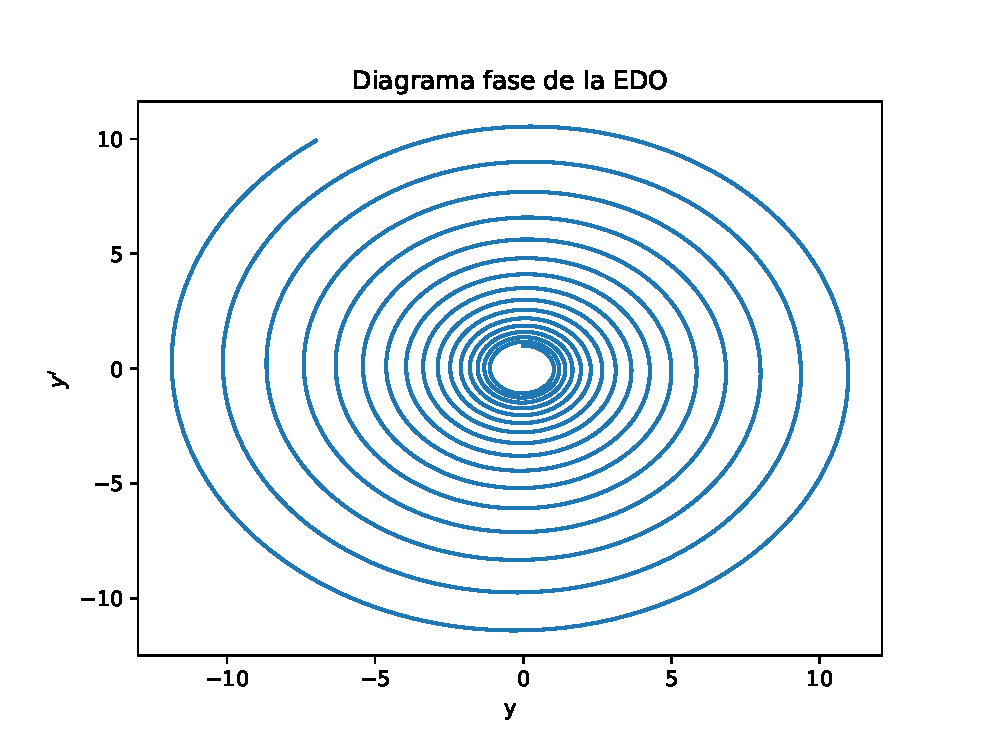
\includegraphics[scale=0.65]{Imagenes/solucion_euler_02.eps}
\end{figure}
\end{frame}
\begin{frame}
\frametitle{Resultado}
El estado fase presenta una trayectoria abierta, por lo que no hay correspondencia con el fenómeno.
\\
\bigskip
El método de Euler no funciona con EDO2 del tipo estudiado.
\end{frame}
\begin{frame}[plain, allowframebreaks, fragile]
\frametitle{Usando el predictor - corrector}
Ahora usaremos el algoritmo de Euler predictor - corrector:
\begin{lstlisting}[caption=Método predictor - corrector, style=FormattedNumber, basicstyle=\linespread{1.1}\ttfamily=\small, columns=fullflexible]
def EulerPC(t, ht, y, n, Func):
   f_1_ = [_0_] * (n + 1)
   f_2_ = [_0_] * (n + 1)
   yt = [_0_] * (n + 1)

   Func(t, y, f_1_)

   for i in range(1, n + 1):
       yt[i] = y[i] + ht * f_1_[i]

   Func(t + ht, yt, f_2_)

   ht_2_ = ht/_2_e_0_
   
   for i in range(1, n + 1):
       y[i] += ht_2_ * (f_1_[i] + f_2_[i])
   
   return y
\end{lstlisting}
\end{frame}
\begin{frame}[fragile]
\frametitle{Cambio en el nombre de archivo}
Ajusta en la línea del código donde se le da un nombre al archivo de datos por lo siguiente:
\begin{verbatim}
open("solucion_euler_pc.txt","w")
\end{verbatim}
\end{frame}
\begin{frame}[fragile]
\frametitle{Ajuste en la graficación}
Realiza el mismo ajuste de nombre de archivo en la línea que abre el archivo de datos:
\begin{verbatim}
open("solucion_euler_pc.txt") as f:
\end{verbatim}
\end{frame}
\begin{frame}[plain]
\frametitle{Solución Euler predictor - corrector}
\begin{figure}
	\centering
	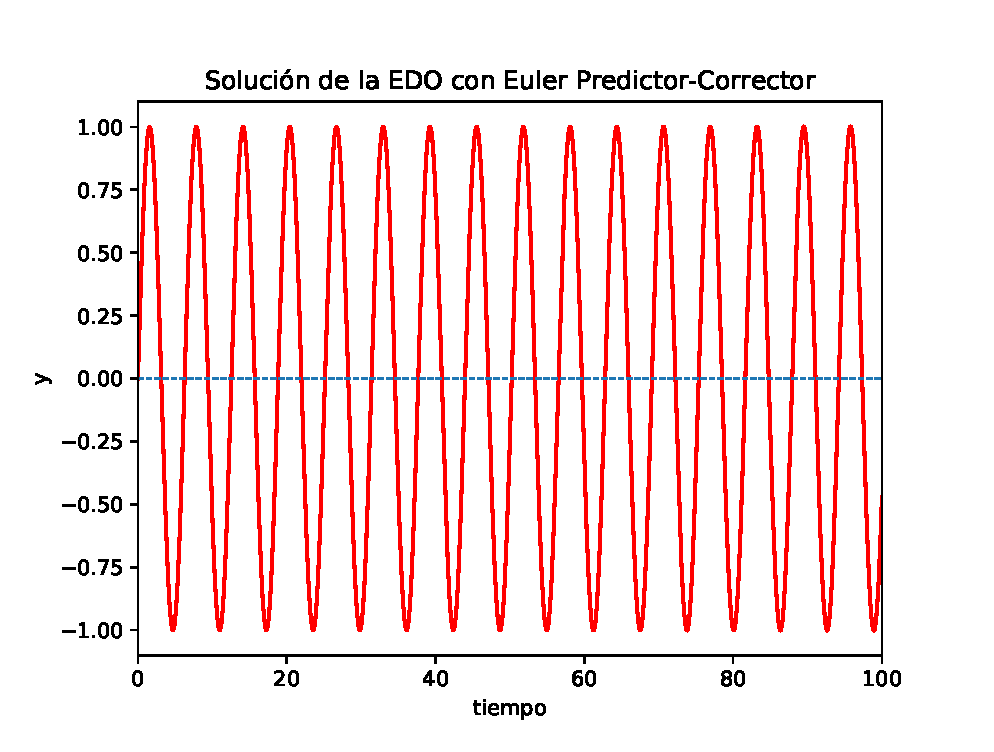
\includegraphics[scale=0.65]{Imagenes/solucion_euler_pc_01.eps}
\end{figure}
\end{frame}
\begin{frame}[plain]
\frametitle{Solución Euler predictor - corrector}
\begin{figure}
	\centering
	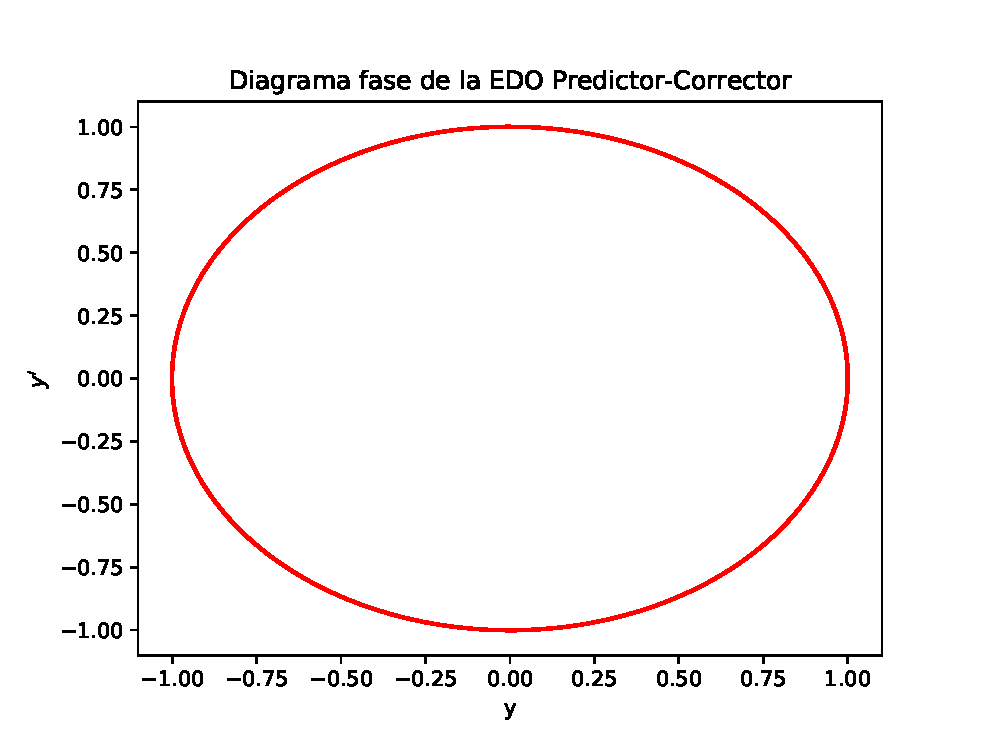
\includegraphics[scale=0.65]{Imagenes/solucion_euler_pc_02.eps}
\end{figure}
\end{frame}
\begin{frame}
\frametitle{Conclusión}
Vemos que el método de Euler predictor - corrector, corrige la falla en la estabilidad de la solución.
\\
\bigskip
Tendrás que revisar si el método permite una solución estable para la EDO.
\end{frame}
\section{Métodos de Runge-Kutta}
\frame{\tableofcontents[currentsection, hideothersubsections]}
\subsection{Objetivo de los métodos Runge-Kutta}
% \begin{frame}
% \frametitle{Métodos de Runge-Kutta}
% Para hacer que el nivel de precisión aumente en el método de Euler, hay que reducir $h$, pero esto genera que se lleve más tiempo en el cálculo y se propague el error por redondeo.
% \end{frame}
% \begin{frame}
% \frametitle{EDO de inicio}
% Sea una EDO:
% \[y^{\prime} =  f(y, t), \hspace{1cm} y(0)= y_{0}\]
% Para calcular $y_{n + 1} = t_{n} + h$ dando un valor de $y_{n}$ se integra la EDO en el intervalo $[t_{n}, t_{n + 1}]$
% \[y_{n + 1} = y_{n} + \int_{t_{n}}^{t_{n + 1}} \: f(y, t) dt\]
% Se resuelve la ecuación del lado derecho mediante integración numérica.
% \end{frame}
% \subsection{Runge-Kutta de segundo orden}
% \begin{frame}
% \frametitle{Runge-Kutta de segundo orden  - RK2}
% Aplicando la regla del trapecio al lado derecho de la ecuación anterior:
% \[\int_{t_{n}}^{t_{n + 1}} f(y,t) \: dt \simeq \dfrac{1}{2} \: h \: [f(y_{n}, t_{n}) + f(y_{n + 1}, t_{n + 1})] \]
% En esta ecuación el término $y_{n + 1}$ es una incógnita, por lo que se aproxima el segundo término mediante $f(y*_{n + 1},t_{n + 1})$ donde $y*_{ + 1}$ es la primera estimación de $y_{n + 1}$ obtenido por el método de Euler hacia adelante.
% \end{frame}
% \begin{frame}
% \frametitle{Runge-Kutta de segundo orden  - RK2}
% \begin{align*}
% y*_{n+1} & = y_{n} + h \: f(y_{n}, t_{n}) \\
% y_{n+1} & = y_{n} + \dfrac{h}{2} [f(y_{n}, t_{n}) + f(y*_{n + 1},t_{n + 1})]
% \end{align*}
% De manera canónica, podemos escribir:
% \begin{align*}
% k_{1} & = h \: f(y_{n}, t_{n}) \\
% k_{2} & = h \: f(y_{n} + k_{1}, t_{n + 1})\\
% y_{n + 1} & = y_{n} + \dfrac{1}{2} \: [k_{1} + k_{2}]
% \end{align*}
% \end{frame}
% \begin{frame}[fragile]
% \frametitle{Ejercicio}
% El circuito que se muestra, tiene una autoinductancia de $L = \SI{50}{\henry}$, una resistencia de $R = \SI{20}{\ohm}$, y una fuente de $V = \SI{10}{\volt}$.
% \begin{figure}
%     \centering
%     \includestandalone{Figuras/circuito_RK2}
%     \caption{Circuito RLC para el ejercicio.}
% \end{figure}
% \end{frame}
% \begin{frame}
% \frametitle{Condiciones iniciales del ejercicio}
% En el tiempo $t = 0$, la corriente $I(t)$ satisface
% \[L \dfrac{d}{dt} I(t) + RI(t) = V, \hspace{1cm} I(0) = 0\]
% Usando el esquema de Runge-Kutta de segundo orden (RK2), calcula la corriente en el circuito para $0\leq t \leq 10$ segundos, con $h = 0.1$
% \end{frame}
% \begin{frame}
% \frametitle{Ajustando la EDO}
% Se reescribe la ecuación como
% \[\dfrac{d}{dt} I = -\dfrac{R}{L} I + \dfrac{V}{L} = f(I, t)\]
% Aplicando el método RK2, tenemos
% \begin{align*}
% k_{1} &= h \: \left[-\dfrac{R}{L} \: I_{n} + \dfrac{V}{L} \right] \\
% k_{2} &= h \left[-\dfrac{R}{L} \: (I_{n} + k_{1}) + \dfrac{V}{L} \right] \\
% I_{n + 1} &= I_{n} + \dfrac{1}{2} \: (k_{1} + k_{2})
% \end{align*}
% \end{frame}
% \begin{frame}[plain, allowframebreaks, fragile]
% \frametitle{Código}
% \fontsize{10}{10}\selectfont
% \begin{lstlisting}[caption=Código para el Ejercicio, style=FormattedNumber, basicstyle=\linespread{1.1}\ttfamily=\small, columns=fullflexible]
% L = 50.0
% R = 20.0
% V = 10.0

% h = 0.1

% corriente = 0
% I = []
% I.append(0)

% for i in range(99):
%     k_1_ = h * ((-R/L) * corriente + (V/L))
%     k_2_ = h *((-R/L) * (corriente + k_1_) + (V/L))
%     corriente = corriente + (k_1_ + k_2_) * 0.5
%     I.append(corriente)
% \end{lstlisting}
% \end{frame}
% \begin{frame}
% \frametitle{Resultado gráfico de la solución}
% La rutina para la gráfica con \funcionazul{matplotlib} la pueden implementar sin mayor problema.
% \end{frame}
% \begin{frame}[fragile]
% \frametitle{Resultado gráfico}
% Nótese que el valor de corriente límite corresponde a $I_{f}=V/R$ que alcanzaría en un tiempo mucho mayor.
% \begin{figure}
% 	\centering
% 	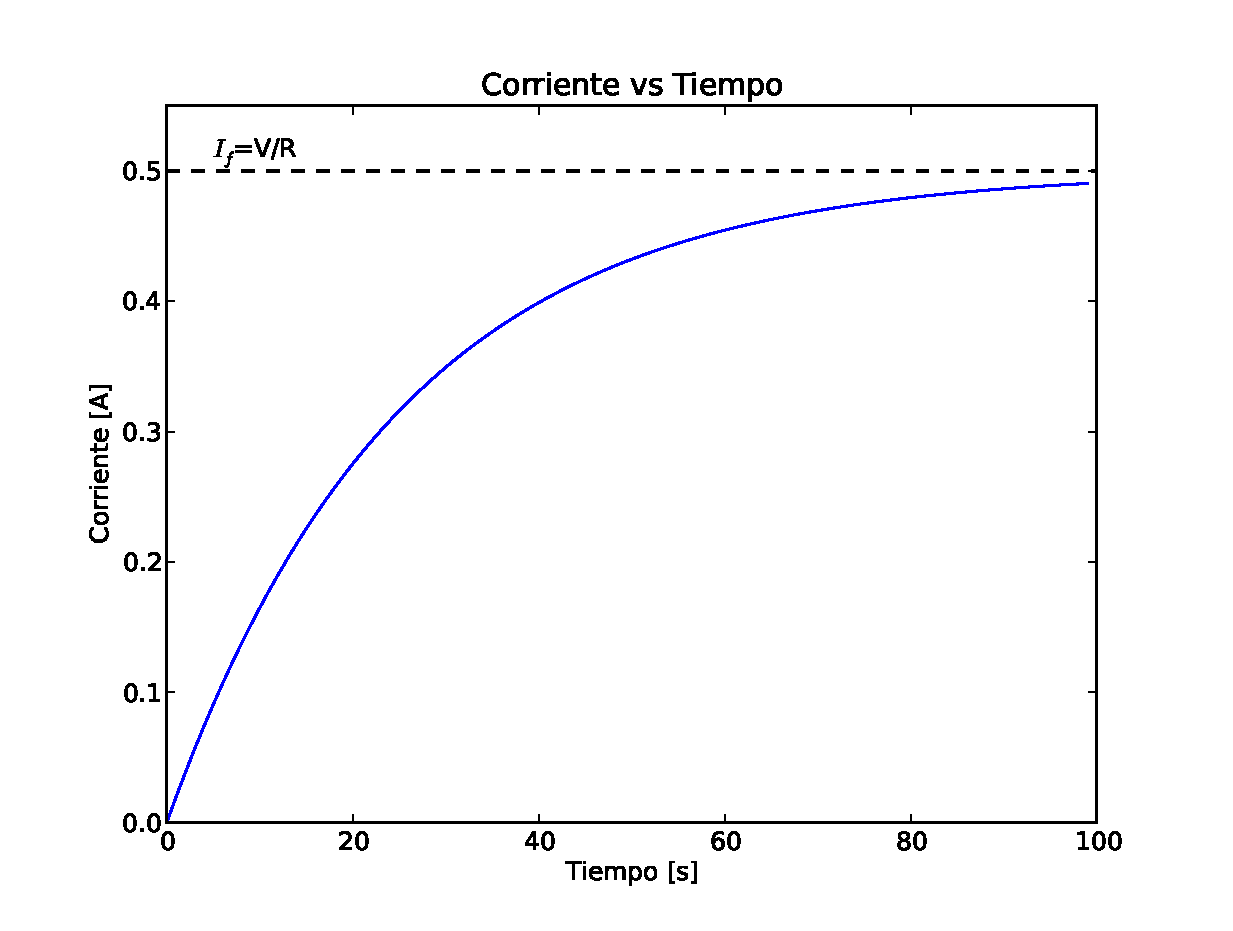
\includegraphics[scale=0.4]{Imagenes/RK2circuito.eps} 
%     \caption{Solución para el circuito, la corriente llega a un límite definido por el valor de $V$ y de $R$.}
% \end{figure}
% \end{frame}
\begin{frame}
\frametitle{Utilidad de los métodos RK}
El objetivo de los métodos de Runge-Kutta (RK) es eliminar la necesidad de la diferenciación repetida de las ecuaciones diferenciales. 
\end{frame}
\begin{frame}
\frametitle{Utilidad de los métodos RK}
Dado que la diferenciación repetida no está implicada en la fórmula de integración en la serie de Taylor de primer orden
\[ \mathbf{y}(x + h) = \mathbf{y}(x) + \mathbf{y}^{\prime}(x) \: h = \mathbf{y}(x) + \mathbf{F}(x,\mathbf{y}) \: h \]
\end{frame}
\section{Método RK1}
\begin{frame}
\frametitle{Método RK1}
Se considera como el método Runge-Kutta de primer orden (RK1), también llamado, \emph{método de Euler}. 
\\
\bigskip
Ya vimos que el error debido al truncamiento es bastante, no se usa en la práctica común.
\end{frame}
\section{Método RK2}
\begin{frame}
\frametitle{Método de Runge-Kutta de segundo orden}
Para obtener el método \azulfuerte{RK2}, suponemos una fórmula de integración del tipo
\fontsize{12}{12}\selectfont
\[ \mathbf{y}(x + h) = \mathbf{y}(x) + c_{0} \: \mathbf{F}(x,\mathbf{y}) \: h + c_{1} \mathbf{F}[x + p \: h, \mathbf{y} + q \: h \mathbf{F}(x, \mathbf{y})] \: h \]
\end{frame}
\begin{frame}
\frametitle{Método de Runge-Kutta de segundo orden}
Debemos de encontrar los parámetros $c_{0}$, $c_{1}$, $p$ y $q$ de tal forma que se parezca a la siguiente serie de Taylor
\begin{align*}
\mathbf{y}(x + h) &= \mathbf{y}(x) + \mathbf{y}^{\prime}(x) \: h + \dfrac{1}{2!}\mathbf{y}^{\prime \prime}(x) \: h^{2} + O(h^{3}) \\
&= \mathbf{y}(x) + \mathbf{F}(x,\mathbf{y}) \: h + \dfrac{1}{2}\mathbf{F}^{\prime}(x,\mathbf{y}) \: h^{2} + O(h^{3})
\end{align*}
\end{frame}
\begin{frame}
\frametitle{Método de Runge-Kutta de segundo orden}
Notemos que
\[ \mathbf{F}^{\prime}(x,\mathbf{y}) = \dfrac{\partial \mathbf{F}}{\partial x} + \sum_{i = 0}^{n - 1} \dfrac{\partial \mathbf{F}}{\partial \mathbf{y}_{i}} \: \mathbf{y}^{\prime}_{i} = \dfrac{\partial \mathbf{F}}{\partial x} + \sum_{i = 0}^{n - 1} \dfrac{\partial \mathbf{F}}{\partial \mathbf{y}_{i}} \: F_{i}(x, \mathbf{y})\]
donde $n$ es el número de \azulfuerte{1-EDO}.
\end{frame}
\begin{frame}
\frametitle{Método de Runge-Kutta de segundo orden}
Entonces podemos escribir para $\mathbf{y}(x + h)$ como
\begin{align*}
\mathbf{y}(x + h) &= \mathbf{y}(x) + \mathbf{F}(x,\mathbf{y}) \: h + \\
&+ \dfrac{1}{2} \left( \dfrac{\partial \mathbf{F}}{\partial x} + \sum_{i=0}^{n-1} \dfrac{\partial \mathbf{F}}{\partial y_{i}} F_{i}(x,\mathbf{y}) \right) h^{2} + O(h^{3})
\end{align*}
\end{frame}
\begin{frame}
\frametitle{Método de Runge-Kutta de segundo orden}
Regresando a la ecuación inicial, re-escribimos el último término mediante una serie de Taylor en varias variables:
\begin{align*}
 \mathbf{F}[x + p \: h, \mathbf{y} &+ q \: h \mathbf{F}(x, \mathbf{y})] = \mathbf{F}(x,\mathbf{y}) + \dfrac{\partial \mathbf{F}}{\partial x} \: p \: h + \\
 &+ q \: h \sum_{i=1}^{n-1} \dfrac{\partial \mathbf{F}}{\partial y_{i}} F_{i}(x,\mathbf{y}) + O(h^{2})
\end{align*}
\end{frame}
\begin{frame}
\frametitle{Método de Runge-Kutta de segundo orden}
Por lo que la ecuación inicial, toma la forma:
\begin{align*}
\mathbf{y}(x &+ h) = \mathbf{y}(x) + (c_{0} + c_{1}) \: \mathbf{F}(x,\mathbf{y}) \: h + \\
&+ c_{1} \left[ \dfrac{\partial \mathbf{F}}{\partial x} \: p \: h + q \: h \sum_{i=1}^{n - 1} \dfrac{\partial \mathbf{F}}{\partial y_{i}} F_{i}(x,\mathbf{y}) \right] h + O(h^{3}) 
\end{align*}
Para que las expresiones sean idénticas, se necesita que:
\[ c_{0} + c_{1} = 1 \hspace{1cm} c_{1} \: p = \dfrac{1}{2} \hspace{1cm} c_{1} \: q = \dfrac{1}{2}\]
\end{frame}
\begin{frame}
\frametitle{Valores de las incógnitas}
El conjunto anterior representa un sistema de tres ecuaciones y cuatro incógnitas, por lo que se asigna un valor a cualquiera de ellas.
\\
\medskip
Las opciones más comunes y sus nombres para los métodos son los siguientes:
\end{frame}
\begin{frame}
\begin{tabular}{| l | l | l | l | l |}
\hline
\multicolumn{4}{|c|}{Valores} & \multicolumn{1}{|c|}{Algoritmo} \\ \hline
$c_{0}= 0$ & $c_{1} = 1$ & $p = \frac{1}{2}$ & $q = \frac{1}{2}$ & Euler modificado \\ \hline
$c_{0} = \frac{1}{2}$ & $c_{1} = \frac{1}{2}$ & $p = 1$ & $q = 1$ & Heun \\ \hline
$c_{0} = \frac{1}{3}$ & $c_{1} = \frac{2}{3}$ & $p = \frac{3}{4}$ & $q = \frac{3}{4}$ & Ralston \\ \hline
\end{tabular}
\\
\medskip
Todas estas fórmulas son del tipo \azulfuerte{RK2}, ninguna tiene una superioridad numérica con respecto a las otras.
\end{frame}
\subsection{Método de Euler modificado}
\begin{frame}
\frametitle{Método de Euler modificado}
Sustituimos los valores de los parámetros en la ecuación general para obtener:
\begin{equation*}
\mathbf{y}(x + h) = \mathbf{y}(x) + \mathbf{F} \left[  x + \dfrac{h}{2}, \mathbf{y} + \dfrac{h}{2} \: \mathbf{F}(x,\mathbf{y}) \right] h
\end{equation*}
\end{frame}
\begin{frame}
\frametitle{Método de Euler modificado}
Esta fórmula de integración puede evaluarse convenientemente, siguiendo la siguiente secuencia de operaciones:
\begin{eqnarray*}
\mathbf{K}_{0} &=& h \mathbf{F}(x,\mathbf{y}) \\
\mathbf{K}_{1} &=& h \mathbf{F} \left( x+\dfrac{h}{2},\mathbf{y}+\dfrac{1}{2} \mathbf{K}_{0} \right) \\
\mathbf{y}(x+h) &=& \mathbf{y}(x) + \mathbf{K}_{1}
\end{eqnarray*}
\end{frame}
\begin{frame}
\frametitle{Rep. del método de Euler modificado}
\begin{figure}
    \centering
    \includestandalone{Figuras/metodo_Euler_modificado}
    \caption{Representación gráfica del método de Euler modificado para una EDO $y^{\prime}=f(x, y)$.}
\end{figure}
\end{frame}
\begin{frame}
\frametitle{Método de Euler modificado}
El valor de $\mathbf{K}_{0}= h \mathbf{F}(x,\mathbf{y})$ devuelve un estimado de $y$ en el punto central para la fórmula de Euler
\[ y(x+\frac{h}{2}) = y(x) + f(x,y) \frac{h}{2} = y(x) + \frac{K_{0}}{2}\]
La segunda ecuación $\mathbf{K}_{1}$, aproxima el área del bloque por el área $K_{1}$ del rectángulo.
\\
\bigskip
El error es proporcional a la curvatura $y^{\prime \prime \prime}$ de la gráfica.
\end{frame}
\begin{frame}
\frametitle{Ejemplo}
Utiliza RK2 para integrar la siguiente EDO:
\[ y^{\prime} = \sin y \hspace{1.5cm} y(0) = 1\]
de $x = 0$ a $x = 0.5$ en pasos de $h=0.1$
\end{frame}
\begin{frame}
\frametitle{Solución}
Del problema tenemos que:
\[ F(x, y) = \sin y\]
por lo que las fórmular canónicas de integración son
\begin{align*}
K_{0} &= h \:  F(x, y) = 0.1 \sin y \\
K_{1} &= h \: F \left( x + \dfrac{h}{2}, y + \dfrac{1}{2} K_{0} \right) = 0.1 \sin \left( y + \dfrac{1}{2} K_{0}\right) \\
y(x + h) &= y(x) + K_{1}
\end{align*}
\end{frame}
\begin{frame}
\frametitle{Solución}
Como $y(0) = 1$, podemos integrar
\begin{align*}
K_{0} &= 0.1 \:  \sin (1.0000) = 0.0841 \\
K_{1} &= 0.1 \: \sin \left( 1.0000 + \dfrac{0.0841}{2} \right)  = 0.0863 \\
y(0.1) &= 1.0 + 0.0863 = 1.0863
\end{align*}
\end{frame}
\begin{frame}
\frametitle{Solución}
En la siguiente evaluación
\begin{align*}
K_{0} &= 0.1 \: \sin (1.0863) = 0.0885 \\
K_{1} &= 0.1 \: \sin \left( 1.0.0863 + \dfrac{0.0885}{2} \right)  = 0.0905 \\
y(0.2) &= 1.0863 + 0.0905 = 1.1768
\end{align*}
y así, sucesivamente.
\end{frame}
\begin{frame}[plain]
\frametitle{Solución}
A manera de resumen, las cuentas se presentan en la siguiente tabla:
\begin{center}
\begin{tabular}{c | c | c | c |}
$x$ & $y$ & $K_{0}$ & $K_{1}$ \\ 
\hline
\hline
$0.0$ & $1.0000$ & $0.0841$ & $0.0863$ \\ \hline
$0.1$ & $1.0863$ & $0.0885$ & $0.0905$ \\ \hline
$0.2$ & $1.1768$ & $0.0923$ & $0.0940$ \\ \hline
$0.3$ & $1.2708$ & $0.0955$ & $0.0968$ \\ \hline
$0.4$ & $1.3676$ & $0.0979$ & $0.0988$ \\ \hline
$0.5$ & $1.4664$ & & \\ \hline
\end{tabular}
\end{center}
\end{frame}
\begin{frame}
\frametitle{Solución}
La solución exacta (que podrían demostrar que cumple) es:
\[ x(y) = ln(\csc y - \cot y) + 0.604582 \]
que devuelve en $x(1.4664) = 0.5000$
\end{frame}
\begin{frame}
\frametitle{Consideraciones}
Sin embargo, es poco probable que esta precisión se mantenga mientras continuemos integrando, dado que los errores (tanto de truncamiento como de redondeo) se van acumulando, si se tiene un rango amplio de integración, se requiere entonces, de mejores fórmulas de integración.
\end{frame}
\begin{frame}[fragile]
\frametitle{Ejercicio}
El circuito que se muestra, tiene una autoinductancia de $L = \SI{50}{\henry}$, una resistencia de $R = \SI{20}{\ohm}$, y una fuente de $V = \SI{10}{\volt}$.
\begin{figure}
    \centering
    \includestandalone{Figuras/circuito_RK2}
    \caption{Circuito RLC para el ejercicio.}
\end{figure}
\end{frame}
\begin{frame}
\frametitle{Condiciones iniciales del ejercicio}
En el tiempo $t = 0$, la corriente $I(t)$ satisface
\[L \dfrac{d}{dt} I(t) + RI(t) = V, \hspace{1cm} I(0) = 0\]
Usando el esquema de Runge-Kutta de segundo orden (RK2), calcula la corriente en el circuito para $0\leq t \leq 10$ segundos, con $h = 0.1$
\end{frame}
\begin{frame}
\frametitle{Ajustando la EDO}
Se reescribe la ecuación como
\[\dfrac{d}{dt} I = -\dfrac{R}{L} I + \dfrac{V}{L} = F(I, t)\]
Aplicando el método RK2, tenemos
\begin{align*}
K_{0} &= h \: \left[-\dfrac{R}{L} \: I_{n} + \dfrac{V}{L} \right] \\
K_{1} &= h \: \left[-\dfrac{R}{L} \: (I_{n} + K_{0}) + \dfrac{V}{L} \right] \\
I_{n + 1} &= I_{n} + \dfrac{1}{2} \: (K_{0} + K_{1})
\end{align*}
\end{frame}
\begin{frame}[plain, allowframebreaks, fragile]
\frametitle{Código}
\begin{lstlisting}[caption=Código para el circuito RLC, style=FormattedNumber, basicstyle=\linespread{1.1}\ttfamily=\small, columns=fullflexible]
L = 50.0
R = 20.0
V = 10.0

h = 0.1

corriente = 0
I = []
I.append(0)

for i in range(99):
    K_0_ = h * ((-R/L) * corriente + (V/L))
    K_1_ = h *((-R/L) * (corriente + k_0_) + (V/L))
    corriente = corriente + (K_0_ + K_1_) * 0.5
    I.append(corriente)
\end{lstlisting}
\end{frame}
\begin{frame}
\frametitle{Resultado gráfico de la solución}
La rutina para la gráfica con \funcionazul{matplotlib} la pueden implementar sin mayor problema.
\end{frame}
\begin{frame}[plain, fragile]
\frametitle{Resultado gráfico}
\begin{figure}
	\centering
	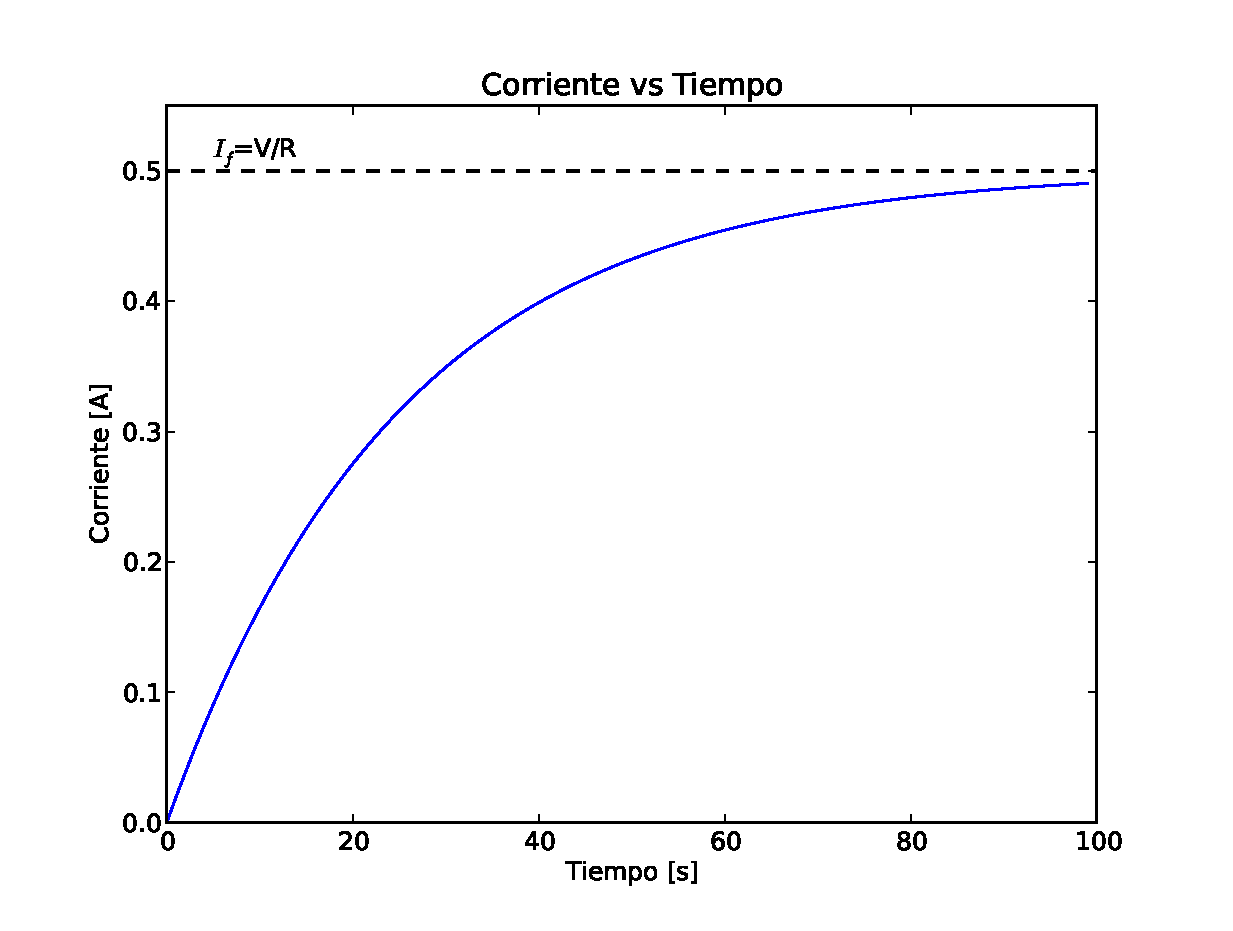
\includegraphics[scale=0.4]{Imagenes/RK2circuito.eps} 
    \caption{Solución para el circuito, la corriente llega a un límite definido por el valor de $V$ y de $R$.}
\end{figure}
\end{frame}
\begin{frame}
\frametitle{Conclusión del ejercicio}
Nótese que el valor de corriente límite corresponde a $I_{f} = V/R$ que alcanzaría en un tiempo mucho mayor.
\end{frame}
\section{Método RK4}
\begin{frame}
\frametitle{Método de Runge-Kutta de cuarto orden}
El método de \azulfuerte{RK4} se obtiene de la serie de Taylor, de la misma forma como se obtuvo RK2; considerando que la derivación es un proceso largo y no tan instructivo, entonces lo omitiremos.
\end{frame}
\begin{frame}
\frametitle{Método de Runge-Kutta de cuarto orden}
La expresión final de la fórmula de integración también depende de la elección de los parámetros, es decir, no hay una única fórmula para \azulfuerte{RK4}.
\end{frame}
\begin{frame}
\frametitle{Método RK4}
La expresión más popular se le conoce como método \azulfuerte{RK4}, que requiere de las siguientes operaciones:
\begin{align*}
K_{0} &= h \: \mathbf{F}(x,\mathbf{y}) \\
K_{1} &= h \: \mathbf{F}(x +\dfrac{h}{2},\mathbf{y} + \dfrac{\mathbf{K}_{0}}{2}) \\
K_{2} &= h \: \mathbf{F}(x +\dfrac{h}{2},\mathbf{y} + \dfrac{\mathbf{K}_{1}}{2}) \\
K_{3} &= h \: \mathbf{F}(x +h, \mathbf{y} + \mathbf{K}_{2}) \\
\mathbf{y}(x+h) &= \mathbf{y}(x) + \dfrac{1}{6} (\mathbf{K}_{0} + 2 \: \mathbf{K}_{1} + 2 \: \mathbf{K}_{2} + \mathbf{K}_{3})
\end{align*}
\end{frame}
\begin{frame}
\frametitle{Método RK4}
El principal inconveniente de este método es que no se presta para una estimación del error de truncamiento. Por lo tanto, tenemos que \enquote{adivinar} el tamaño del paso de integración $h$, o determinarlo por ensayo y error.
\end{frame}
\begin{frame}
\frametitle{Alternativa: métodos adaptativos}
En contraste, los llamados métodos adaptativos pueden evaluar el error de truncamiento en cada paso de integración y ajustar el valor de $h$ en consecuencia, pero con un gran costo, computacionalmente hablando.
\end{frame}
\subsection{Algoritmo RK4}
\begin{frame}
\frametitle{Algoritmo RK4}
La función \azulfuerte{\texttt{integra}} en este módulo, implementa el método \azulfuerte{RK4}.
\\
\bigskip
El usuario deberá de proporcionar en \azulfuerte{\texttt{integra}} la función \texttt{F(x,y)} que define el conjunto de \textoazul{1-EDO} $\mathbf{y}^{\prime} = \mathbf{F}(x,\mathbf{y})$. 
\end{frame}
\begin{frame}[plain, allowframebreaks, fragile]
\begin{lstlisting}[caption=Código para la función integra, style=FormattedNumber, basicstyle=\linespread{1.1}\ttfamily=\small, columns=fullflexible]
def integra(F, x, y, xAlto, h):
    
    def rk_4_(F, x, y, h):
        K_0_ = h * F(x,y)
        K_1_ = h * F(x + h/2.0, y + K_0_/2.0)
        K_2_ = h * F(x + h/2.0, y + K_1_/2.0)
        K_3_ = h * F(x + h, y + K_2_)
        
        return (K_0_ + 2.0 * K_1_ + 2.0 * K_2_ + K_3_) / 6.0
    
    X = []
    Y = []
    X.append(x)
    Y.append(y)

    while x < xAlto:
        h = min(h, xAlto - x)
        y = y + rk_4_(F, x, y, h)
        x = x + h
        X.append(x)
        Y.append(y)
    
    return array(X), array(Y)
\end{lstlisting}
\end{frame}
\begin{frame}
\frametitle{Ejemplo}
Resolver
\[ y^{\prime \prime} = -0.1 \: y^{\prime} - x \hspace{1.5cm} y(0) = 0 \hspace{1cm} y^{\prime}(0)=1\]
de $x = 0$ a $x = 2$ con incrementos de $h = 0.25$ mediante \azulfuerte{RK4}.
\end{frame}
\begin{frame}
\frametitle{Solución}
Usando la notación $y_{0} = y$ junto con $y_{1} = y'$, podemos escribir un conjunto de \azulfuerte{1-EDO} como
\begin{equation*} 
\mathbf{y}^{\prime} = \mathbf{F}(x,\mathbf{y}) =
\begin{bmatrix}
y^{\prime}_{0} \\
y^{\prime}_{1}
\end{bmatrix} = 
\begin{bmatrix}
y_{1} \\

\end{bmatrix}
\end{equation*}
\end{frame}
\begin{frame}[plain, allowframebreaks, fragile]
\frametitle{Código completo}
\begin{lstlisting}[caption=Código para el ejercicio, style=FormattedNumber, basicstyle=\linespread{1.1}\ttfamily=\small, columns=fullflexible]
def F(x,y):
    F = zeros((2), dtype='float_64_')
    F[_0_] = y[_1_]
    F[_1_] = -0.1 * y[_1_] - x
    return F

x = 0.0
xAlto = 2.0
y = array([0.0,1.0])
h = 0.25
freq = 1

X,Y = integra(F, x, y, xAlto, h)
imprimeSoln(X, Y, freq)
\end{lstlisting}
\end{frame}
\begin{frame}[plain]
\frametitle{Resultado}
\fontsize{10}{10}\selectfont
\begin{center}
\begin{tabular}{c | c | c }
$x$ & $y[0]$ & $y[1]$ \\ \hline
$0.0000e+00$ & $0.0000e+00$ & $1.0000e+00$ \\ \hline   
$2.5000e-01$ & $2.4431e-01$ & $9.4432e-01$ \\ \hline 
$5.0000e-01$ & $4.6713e-01$ & $8.2829e-01$ \\ \hline
$7.5000e-01$ & $6.5355e-01$ & $6.5339e-01$ \\ \hline
$1.0000e+00$ & $7.8904e-01$ & $4.2110e-01$ \\ \hline
$1.0000e+00$ & $7.8904e-01$ & $4.2110e-01$ \\ \hline
$1.0000e+00$ & $7.8904e-01$ & $4.2110e-01$ \\ \hline
$1.2500e+00$ & $8.5943e-01$ & $1.3281e-01$ \\ \hline
$1.5000e+00$ & $8.5090e-01$ & $2.1009e-01$ \\ \hline 
$1.7500e+00$ & $7.4995e-01$ & $6.0625e-01$ \\ \hline 
$2.0000e+00$ & $5.4345e-01$ & $-1.0543e+00$ \\ \hline 
\end{tabular}
\end{center}
\end{frame}
\begin{frame}
\frametitle{Ejercicio 2}
Usa \textoazul{RK4} para integrar
\[ y^{\prime} = 3 \: y - 4 \: e^{-x} \hspace{1.5cm} y(0)=1 \]
desde $x = 0$ hasta $x = 10$ en pasos de $h = 0.1$. 
\\
\bigskip
Compara el resultado con la solución analítica $y = \exp(-x)$
\end{frame}
\begin{frame}
\frametitle{Solución al ejercicio}
Usaremos el programa anterior. Recordemos que la función \azulfuerte{\texttt{rk\_4}} supone que $y$ es un arreglo, por lo que debemos de especificar la condición inicial como $y = \text{array}([1.0])$ y no $y=1.0$
\end{frame}
\begin{frame}[plain, allowframebreaks, fragile]
\begin{lstlisting}[caption=Código para el ejercicio, style=FormattedNumber, basicstyle=\linespread{1.1}\ttfamily=\small, columns=fullflexible]
def F(x,y):
    F = zeros((1), dtype='float_64_')
    F[_0_] = 3.0 * y[_0_] - 4.0 * exp(-x)
    return F


x = 0.0
xAlto = 10.0
y = array([1.0])
h = 0.1
freq = 20

X,Y = integra(F, x, y, xAlto, h)
imprimeSoln(X, Y, freq)
\end{lstlisting}
\end{frame}
\begin{frame}
\frametitle{Resultado}
\begin{center}
\begin{tabular}{c | c }
$x$  &  $y[0]$ \\ \hline 
$0.0000e+00$ & $1.0000e+00$ \\ \hline
$2.0000e+00$ & $1.3250e-01$ \\ \hline
$4.0000e+00$ & $-1.1237e+00$ \\ \hline
$6.0000e+00$ & $-4.6056e+02$ \\ \hline
$8.0000e+00$ & $-1.8575e+05$ \\ \hline
$1.0000e+01$ & $-7.4912e+07$
\end{tabular}
\end{center}
\pause
\textcolor{red}{Pero ¿es correcto esto?}
\end{frame}
\begin{frame}
\frametitle{¿Qué ocurrió?}
De acuerdo a la solución numérica, $y$ debería de acercarse a cero conforme se incrementa $x$, pero el resultado nos muestra lo contrario: después de un incremento inicial, la magnitud de $y$ se incrementa súbitamente.
\\
\bigskip
Podemos explicar esto mirando de cerca la solución analítica.
\end{frame}
\begin{frame}
\frametitle{Solución general}
La solución general de la EDO dada es
\[ y = C \: e^{3\: x} + e^{-x} \]
que puede verificarse por sustitución.
\\
\medskip
La condición inicial $y(0) = 1$ hace que $C = 0$, que para la solución del problema, es precisamente $y = exp(-x)$.
\end{frame}
\begin{frame}
\frametitle{Solución general}
El problema en la solución numérica es el término dominante $C \: e^{3 \: x}$
\\
\medskip
Supongamos que la condición inicial tiene un pequeño error $\varepsilon$, por lo que tenemos $y(0) = 1 + \varepsilon$.
\\
\bigskip
Esto cambia la solución analítica por
\[ y = \varepsilon e^{3 \: x} + e^{-x} \]
\end{frame}
\begin{frame}
\frametitle{Solución general}
\[ y = \varepsilon e^{3 \: x} + e^{-x} \]
Vemos que el término que contiene el error $\varepsilon$, se hace dominante conforme $x$ aumenta. 
\end{frame}
\begin{frame}
\frametitle{Sensibilidad de las condiciones iniciales}
Dado que los errores son inherentes a las soluciones numéricas, tenemos el mismo efecto para cambios pequeños en las condiciones iniciales.
\\
\bigskip
Concluimos que nuestra solución numérica es víctima de la \emph{\textcolor{red}{inestabilidad numérica}}, debida a la sensibilidad de la solución a las condiciones iniciales.
\end{frame}
\end{document}